\chapter{The Trigger \& Data Acquisition}

	The Trigger system within ATLAS is designed to manage the high rate of events produced by the LHC and bring it down to a rate that events can be written to permanent storage by selecting ``interesting'' events. The related Data Acquisition (DAQ) system controls the flow of data from detector hardware through the trigger system to permanent storage at CERN and the worldwide tier 1 grid sites. 

	The Trigger system is made up of three main decision levels; Level 1, Level 2 and Event Filter. Level 1 (L1) is mainly hardware based using limited detector information to locate regions of interest (RoI's)and pass them higher up. The Level 2 (L2) system checks the RoIs with full detector granularity and precision and the last stage the Event Filter (EF) uses analysis reconstruction techniques to further select ``interesting'' events down to the level of 400-500 Hz in 2012. Both the L2 and EF triggers compose what is called the High-Level-Trigger (HLT) together with the event building software needed by the EF.

	(- CTP central trigger processor)
	(- trigger diagram or data flow)

	Following is a description of each of the sections of the trigger while focusing in on the selection of electron objects that are relevant for this analysis. Following this is a discussion of how the trigger menu is formed so bandwidth can be shared between the differing physics goals as well as how ATLAS handles the continued high luminosity push of the LHC.


\section{Level-1 Trigger}

	The Level 1 (L1) trigger searches for regions of interest (RoI's) consisting of strong signatures, ie. high $p_{T}$, muons, electron/photons or jets. The L1 trigger also searches from events with a large missing transverse energy ($E^{miss}_{T}$) or large total transverse energy ($\Sigma E_{T}$). Due to the speed required of a decision only some parts of the detector can be used at L1 and at a much coarser granularity than is possible. For muon acceptance only the RPC's and TGC's can be used while for electromagnetic clusters and jets as well as large $E^{miss}_{T}$ and $\Sigma E_{T}$ the full calorimetry system can be used. The Inner Detector can not be used in L1 decisions due to the time constraint.


	(- timing constraint, 50 ns bunch crossing, latency less than \SI{2.5}{\us}, target \SI{2.0}{\us} with about \SI{1.0}{\us} accounted for by cable propagation.)
	(- pipeline memories)
	(- where and what these calculations are carried out on?)

	The L1Calo system uses trigger towers with a granularity reduced to roughly $0.1 \times 0.1$ in $\Delta\eta \times \Delta\phi$ in most of the detector range from both the electromagnetic and hadronic calorimeters. The ECAL produces almost 3500 of these trigger towers via summation of the analogue signals from a range of trigger cells. This trigger tower data is then sent to the Cluster Processor (CP) to identify electron/photon and tau candidates with $E_{T}$ above a required threshold and passing isolation requirements which are labelled as RoI's.

	\begin{figure}[h]

		\begin{center}
			$\vcenter{\hbox{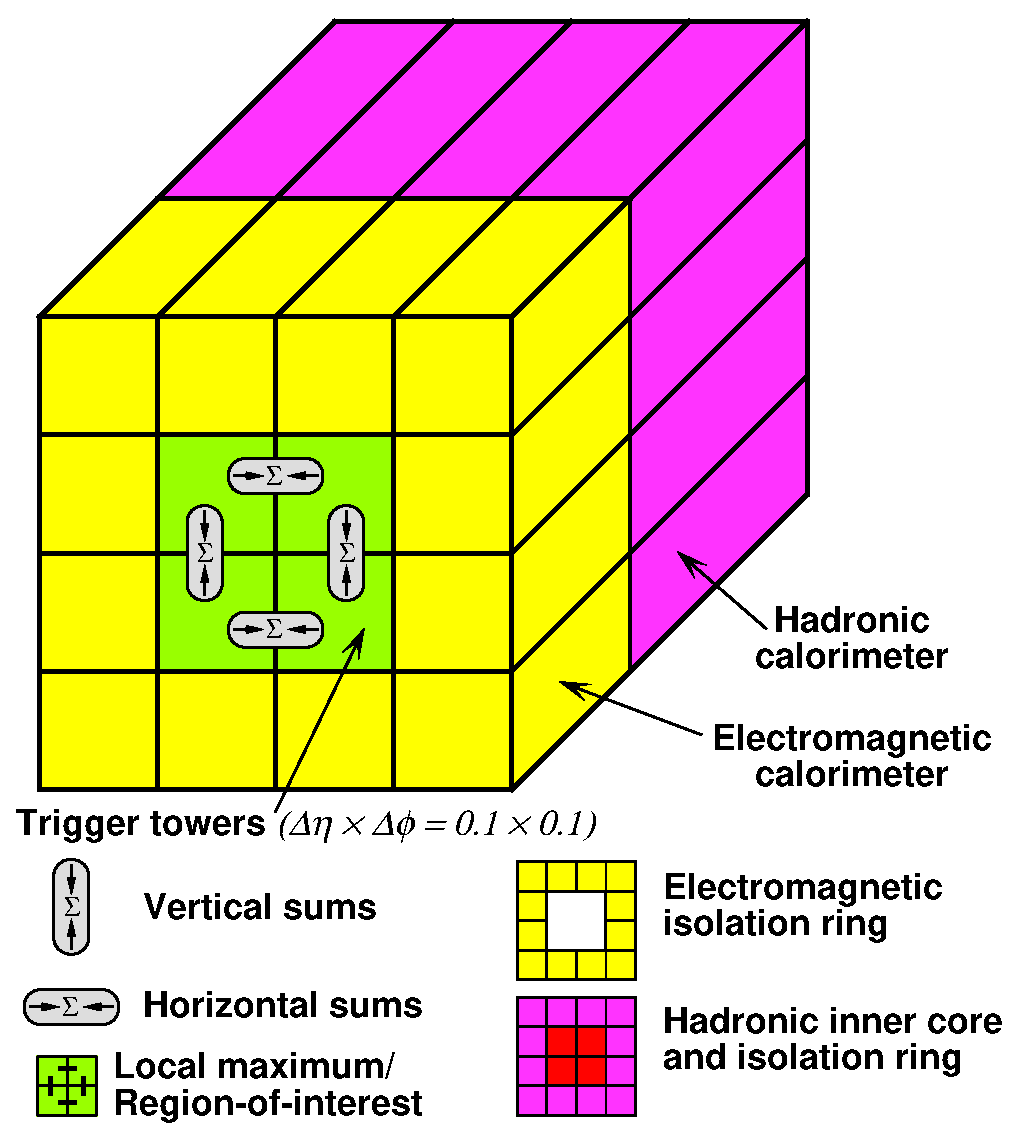
\includegraphics[scale=0.5]{images/EGammaTauAlgo.eps}}}$
			\hspace*{.5in}
			$\vcenter{\hbox{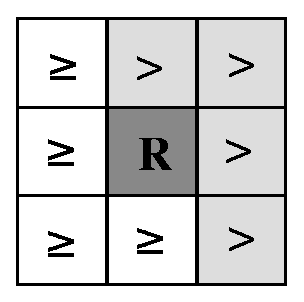
\includegraphics[scale=1.3]{images/LocalMax.eps}}}$
		\end{center}
		\caption{ Electron/photon and tau trigger algorithms (Left) and ET local-maximum test for a cluster/RoI candidate (Right). (The eta-axis runs from left to right, and the phi-axis from bottom to top. The symbol R refers to the candidate 2x2 region being tested.)  }
		\label{fig:Trig_algo}
	\end{figure}


	Figure \ref{fig:Trig_algo} shows how the electron/photon trigger clustering algorithm works by identifying $2 \times 2$ clusters of trigger towers within which two adjacent towers sum to greater than the triggering threshold defined in the trigger menu (seen in section \ref{sec:trig_menu}). Also shown is how three forms of isolation can be applied at this stage; the 12-tower surrounding ring, the $2 \times 2$ hadronic core behind the RoI and the 12-tower surrounding ring in the hadronic calorimeter. Only the hadronic core isolation has so far been used in electron/photon trigger's within ATLAS so far. 
	As all possible $2 \times 2$ clusters are observed in this way it is possible to have double counting of RoIs and so sum of each $2 \times 2$ RoI must be greater than each of its eight nearest overlapping neighbours. Figure \ref{fig:Trig_algo} also shows how this local-maxima is tested while avoiding identical sums through use of `greater than' and `greater than or equal to' in differing $\eta$ and $\phi$ directions. 
	After these clusters have passed the thresholds set it is these RoI's which are passed on the next level of the trigger as a seed to its calculations.





\section{Level-2 Trigger}




\section{Event Filter}





\section{Data Acquisition}




\section{Trigger Menu and Rates}
\label{sec:trig_menu}

\subsection{The ``$e/\gamma$'' Trigger Menu} 














\subsection{Trigger Rates in High Luminosity Regime}

	The ATLAS trigger system comprises a
	hardware-based Level-1 (L1) trigger and a software-based
	High Level Trigger (HLT), subdivided into the Level-2
	(L2) and Event Filter (EF). Due to the bandwidth
	limitations of the trigger each level is restricted to a
	certain output rate. During 2011 the L1 output rate was
	kept below 60 kHz, L2 below 5 kHz and the EF output
	rate at around 400 Hz averaged over the LHC fills. The
	bandwidth allocated to the $e/\gamma$ triggers was
	approximately 30\% of the total EF output rate.
	Electron and photon identification is accomplished by a
	set of $\eta$- and $E_{T}$-dependent rectangular cuts variables
	\cite{trig1, trig2}.\\
	Throughout 2011 data taking at ATLAS the luminosity continued to increase putting pressure on the trigger's ability to control the output rate. Several methods were employed to reduce the trigger rate and in the $e/\gamma$ trigger a variable threshold and hadronic core isolation was investigated to reduce the rate of the Level-1 trigger. In order to keep within time constraints only a coarse granularity is available Level-1 trigger in regions of 0.4 $\eta$. Threshold requirements were therefore investigated varying every 0.4 $\eta$. The effect of a hadronic core isolation was also investigated on the selection of electrons which defines a region in the hadronic calorimeter behind the $e/\gamma$ candidate in which you require and minimum amount of energy to be deposited to distinguish between jets and $e/\gamma$ objects. 


	\begin{figure}[h!]
		\centering
			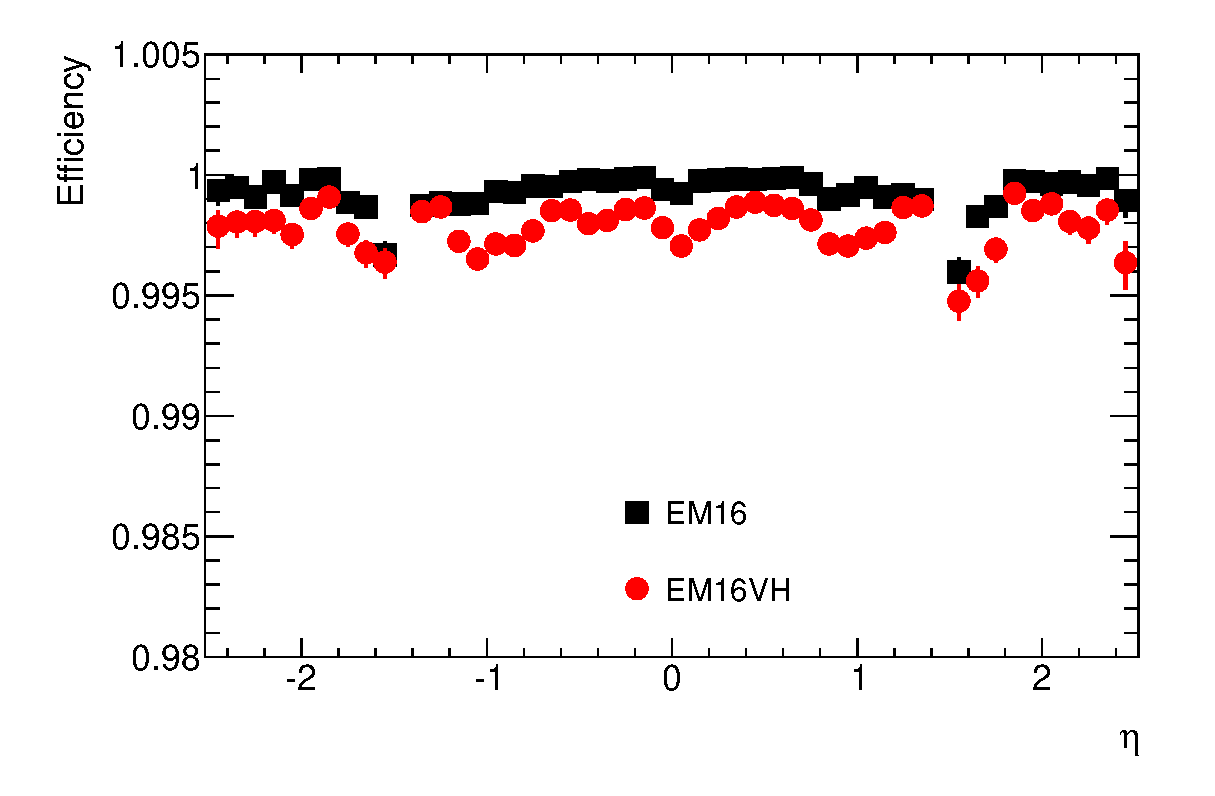
\includegraphics[width=0.49\linewidth]{images/L1_EM16VH_TandP_eff_vs_eta.eps}
			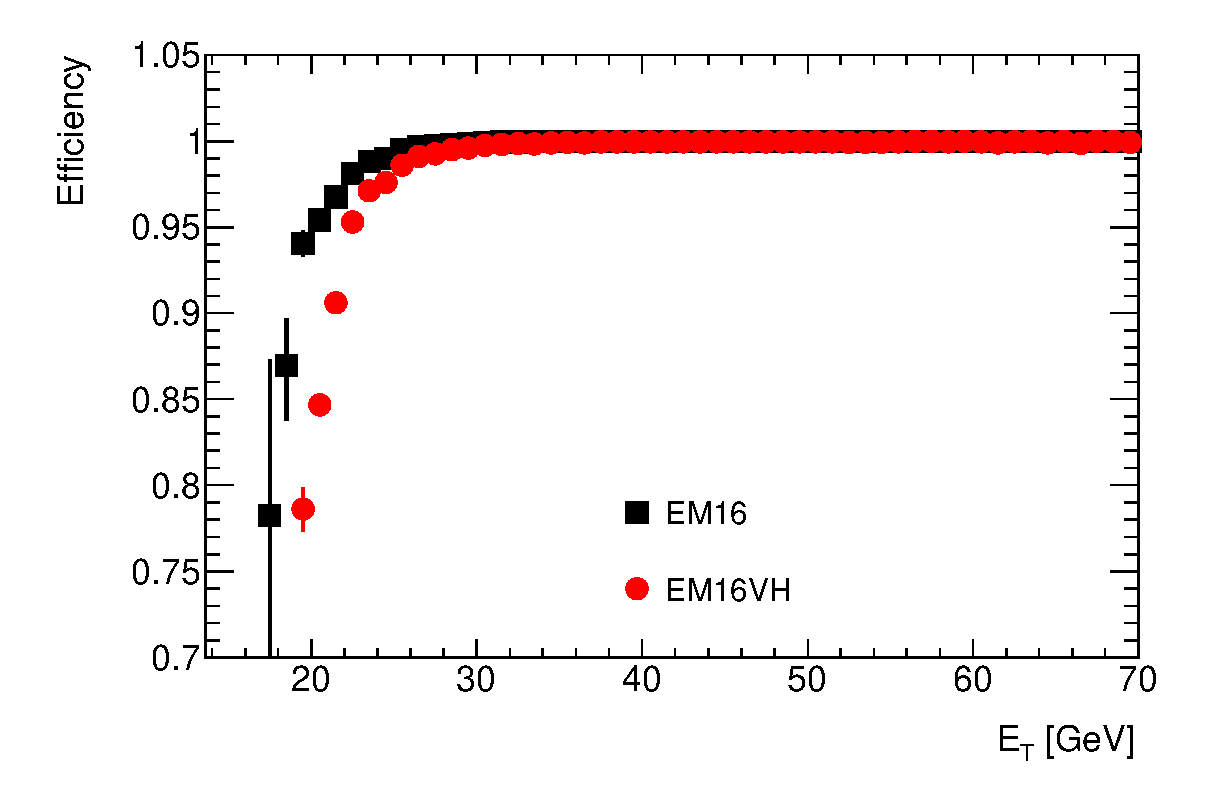
\includegraphics[width=0.49\linewidth]{images/L1_EM16VH_TandP_eff_vs_Et.eps}

			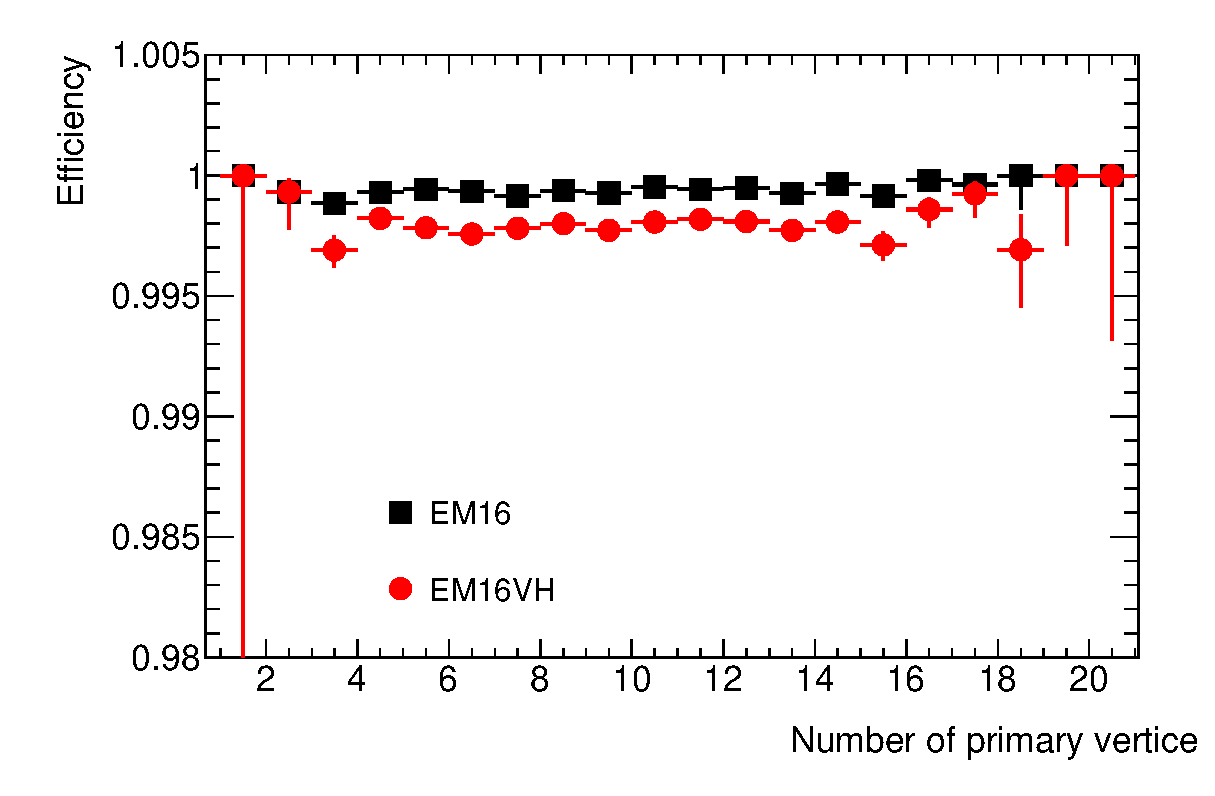
\includegraphics[width=0.49\linewidth]{images/L1_EM16VH_TandP_eff_vs_pvx.eps}
		\caption{Performance of the first level of the ATLAS $e/\gamma$ trigger before(EM16) and after(EM16VH) variable thresholds and hadronic core isolation are applied.}
		\label{fig:L1}
	\end{figure}

	These attempts where successful and rate reduced to compensate for the high luminosity environment. Fig. \ref{fig:L1} shows the performance of the trigger after these changes had been made. It can be seen that a minimal impact of these new requirements is felt.


	There was also a contribution to the maintenance of the $e/\gamma$ trigger software run in the ATLAS detector, both these tasks forming the authorship qualification. The authorship task culminated in presentation of a poster on behalf of the $e/\gamma$ trigger group at the Computing and High Energy Physics (CHEP) conference held New York in May 2012. The contribution is included two pages previously and details the performance of the $e/\gamma$ trigger in the 2011 run period \cite{poster}.

